\documentclass[10pt]{beamer}

\usetheme{Madrid}
\usecolortheme{default}

\usepackage{graphicx}
\usepackage{amsmath}
\usepackage{subfig}
\usepackage{booktabs}
\usepackage{textcomp}
\usepackage{siunitx}

\title[DECT-2020 NR Latency Analysis]{Measurement-Driven Latency Analysis of Uplink/Downlink Scheduling in DECT-2020 NR}

\author[A. Alizai et al.]{
Ashuqullah Alizai 
}

\institute[Aalen University]{
Aalen University of Applied Sciences\\
Aalen, Germany
}

\date{IEEE Conference Presentation}

\begin{document}

%------------------------------------------------
\begin{frame}
\titlepage
\end{frame}

%------------------------------------------------
\begin{frame}{Outline}
\tableofcontents
\end{frame}

%------------------------------------------------
\section{Motivation}

\begin{frame}{Motivation}
\begin{itemize}
    \item DECT-2020 NR is an ETSI-standardized non-cellular 5G radio technology.
    \item It targets low-latency private and industrial wireless networks.
    \item Existing studies report promising end-to-end latency.
    \item However, most results do not decompose latency sources.
    \item RX--TX turnaround and UL/DL scheduling effects remain insufficiently quantified.
\end{itemize}
\end{frame}

%------------------------------------------------
\begin{frame}{Problem Statement}
\begin{block}{Main Problem}
In single-transceiver DECT-2020 NR platforms, uplink and downlink cannot occur simultaneously.
\end{block}

\begin{itemize}
    \item UL/DL alternation requires transceiver reconfiguration.
    \item This creates RX--TX turnaround delay.
    \item The delay becomes important for short-packet and request--response traffic.
    \item Scheduling decisions determine how frequently this delay accumulates.
\end{itemize}
\end{frame}

%------------------------------------------------
\section{Objectives}

\begin{frame}{Research Objectives}
\begin{enumerate}
    \item Quantify RX--TX turnaround delay in a practical DECT-2020 NR implementation.
    \item Analyze how UL/DL scheduling affects end-to-end latency.
    \item Compare sequential and grouped uplink scheduling scenarios.
    \item Identify whether latency is mainly limited by scheduling or hardware constraints.
    \item Discuss design directions for future low-latency DECT-2020 NR systems.
\end{enumerate}
\end{frame}

%------------------------------------------------
\section{System Model}

\begin{frame}{Industrial Sensor--Actuator Star Topology}
\begin{figure}
\centering
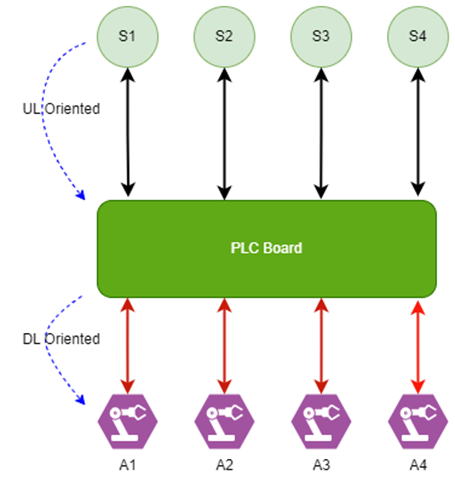
\includegraphics[width=0.50\linewidth]{SandAC.png}
\caption{Industrial sensor--actuator communication model using DECT-2020 NR star topology.}
\end{figure}
\end{frame}

%------------------------------------------------
\begin{frame}{System Model}
\begin{itemize}
    \item A PLC acts as the Fixed Termination node.
    \item Sensors and actuators operate as Portable Termination nodes.
    \item Sensor nodes transmit data in uplink.
    \item Actuator nodes receive control commands in downlink.
    \item Direct PT-to-PT communication is not considered.
\end{itemize}

\begin{block}{Topology}
Star topology coordinated by the FT node.
\end{block}
\end{frame}

%------------------------------------------------
\begin{frame}{Communication Model}
\begin{itemize}
    \item DECT-2020 NR uses Time Division Duplexing.
    \item UL and DL share the same frequency resources.
    \item Transmission directions are separated in time.
    \item The FT node switches between RX and TX states.
    \item The switching delay is implementation-dependent.
\end{itemize}
\end{frame}

%------------------------------------------------
\begin{frame}{Latency Components}
End-to-end latency is decomposed into:

\begin{equation}
L_{\mathrm{E2E}} =
L_{\mathrm{sched}} +
L_{\mathrm{turnaround}} +
L_{\mathrm{PHY}}
\end{equation}

\begin{itemize}
    \item $L_{\mathrm{sched}}$: MAC scheduling and queuing delay
    \item $L_{\mathrm{turnaround}}$: RX--TX transceiver switching delay
    \item $L_{\mathrm{PHY}}$: physical-layer transmission time
\end{itemize}

\begin{alertblock}{Focus}
This work focuses on RX--TX turnaround and its interaction with UL/DL scheduling.
\end{alertblock}
\end{frame}

%------------------------------------------------
\section{Experimental Setup}

\begin{frame}{Experimental Setup}
\begin{figure}
\centering
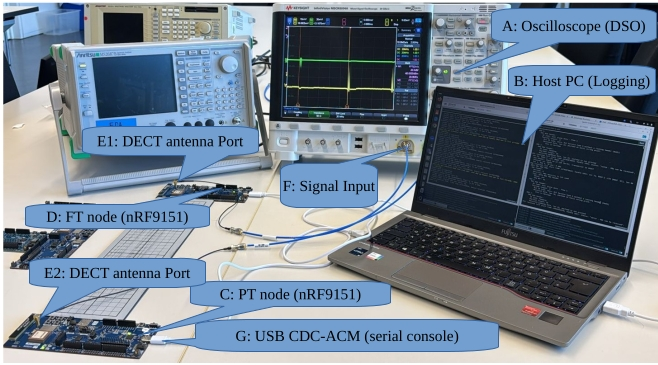
\includegraphics[width=0.85\linewidth]{main_setup.jpg}
\caption{Laboratory setup for RX--TX turnaround measurement using two nRF9151 nodes and DSO.}
\end{figure}
\end{frame}

%------------------------------------------------
\begin{frame}{Hardware Platform}
\begin{itemize}
    \item Two DECT-2020 NR nodes were used.
    \item Both nodes were based on the Nordic Semiconductor nRF9151 SoC.
    \item One node was configured as FT.
    \item One node was configured as PT.
    \item The platform uses a single RF transceiver chain.
\end{itemize}

\begin{block}{Important Limitation}
The platform cannot receive and transmit simultaneously.
\end{block}
\end{frame}

%------------------------------------------------
\begin{frame}{Measurement Method}
\begin{itemize}
    \item GPIO timing markers were generated by firmware.
    \item Markers indicated RX completion and TX start events.
    \item A Digital Storage Oscilloscope captured these markers.
    \item Internal modem timing was also collected.
    \item The \texttt{dect\_shell} reference application was used with minimal instrumentation.
\end{itemize}
\end{frame}

%------------------------------------------------
\begin{frame}{Measurement Procedure}
\begin{enumerate}
    \item FT and PT exchanged predefined UL/DL traffic.
    \item RX completion marker was captured.
    \item TX start marker was captured.
    \item RX--TX turnaround was calculated as:
\end{enumerate}

\begin{equation}
T_{\mathrm{turnaround}} =
T_{\mathrm{TX,start}} -
T_{\mathrm{RX,complete}}
\end{equation}

\begin{itemize}
    \item Multiple RX--TX transitions were measured.
    \item Measurements were repeated to verify consistency.
\end{itemize}
\end{frame}

%------------------------------------------------
\section{Scheduling Scenarios}

\begin{frame}{UL Scheduling Scenarios}
\begin{figure}
\centering
\subfloat[Sequential UL scheduling]{
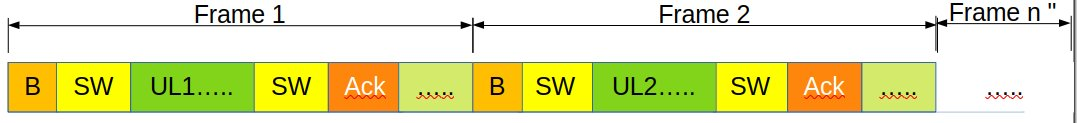
\includegraphics[width=0.47\linewidth]{scenario1.jpg}}
\hfill
\subfloat[Grouped UL scheduling]{
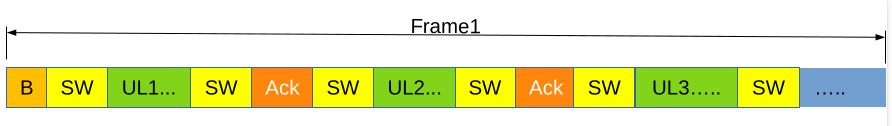
\includegraphics[width=0.47\linewidth]{scenario2.jpg}}
\caption{Sequential and grouped UL scheduling scenarios.}
\end{figure}
\end{frame}

%------------------------------------------------
\begin{frame}{Scenario 1: Sequential UL Scheduling}
\begin{itemize}
    \item UL transmissions are scheduled sequentially across frames.
    \item Each UL transmission is followed by a DL acknowledgment.
    \item This causes frequent UL/DL alternation.
    \item RX--TX turnaround occurs repeatedly.
\end{itemize}

\begin{alertblock}{Expected Effect}
Latency increases strongly as the number of UL transmissions increases.
\end{alertblock}
\end{frame}

%------------------------------------------------
\begin{frame}{Scenario 1 Latency Model}
For sequential uplink scheduling:

\begin{equation}
L_{n}^{(1)} =
\frac{7~\mathrm{slots} + T_{\mathrm{data}}^{UL_x}}
{10~\mathrm{ms}}
=
\frac{2.9~\mathrm{ms} + T_{\mathrm{data}}^{UL_x}}
{10~\mathrm{ms}}
\end{equation}

\begin{itemize}
    \item Each UL transmission incurs approximately seven slots of overhead.
    \item This corresponds to about 2.9 ms.
    \item The latency includes fixed scheduling overhead and payload transmission time.
\end{itemize}
\end{frame}

%------------------------------------------------
\begin{frame}{Scenario 2: Grouped UL Scheduling}
\begin{itemize}
    \item Multiple UL transmissions are grouped in one frame.
    \item Scheduling overhead is shared across several packets.
    \item This reduces frame-level coordination overhead.
    \item However, acknowledgments still require RX--TX switching.
\end{itemize}

\begin{block}{Main Observation}
Grouping helps, but turnaround-induced latency remains significant.
\end{block}
\end{frame}

%------------------------------------------------
\begin{frame}{Scenario 2 Latency Model}
For grouped uplink scheduling:

\begin{equation}
L_{n}^{(2)} =
\frac{19~\mathrm{slots} + T_{\mathrm{data}}^{UL_{1,2,3}}}
{10~\mathrm{ms}}
=
\frac{7.9~\mathrm{ms} + T_{\mathrm{data}}^{UL_{1,2,3}}}
{10~\mathrm{ms}}
\end{equation}

\begin{itemize}
    \item Three UL transmissions incur approximately nineteen slots of overhead.
    \item Combined UL payload occupies about four slots.
    \item Grouping amortizes scheduling overhead across multiple packets.
\end{itemize}
\end{frame}

%------------------------------------------------
\section{Results}

\begin{frame}{Measured Latency Results}
\begin{figure}
\centering
\subfloat[Scenario 1]{
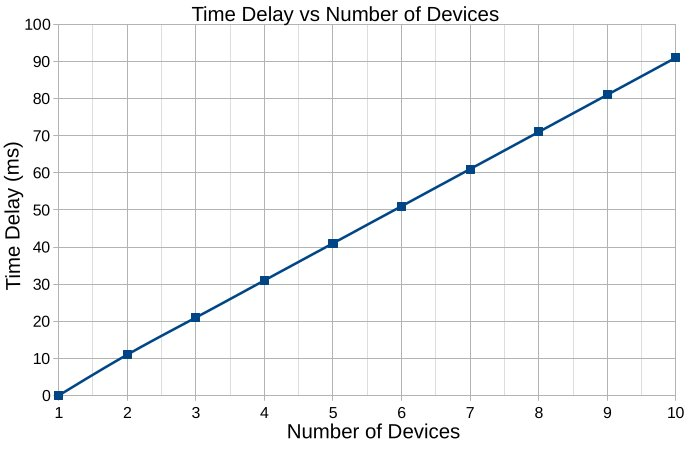
\includegraphics[width=0.47\linewidth]{s1graph.jpg}}
\hfill
\subfloat[Scenario 2]{
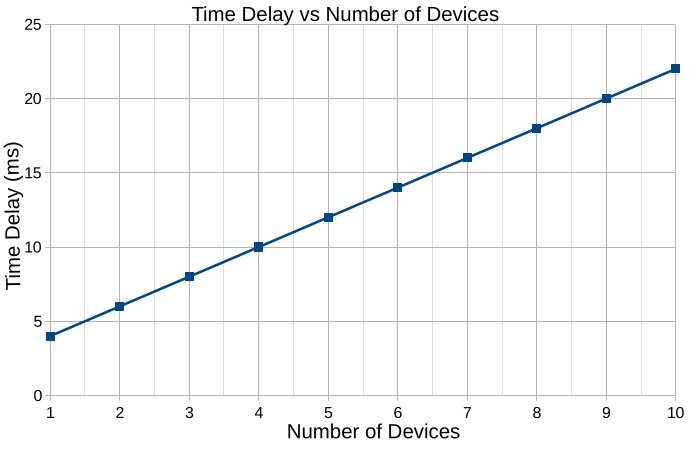
\includegraphics[width=0.47\linewidth]{s2graph.jpg}}
\caption{Measured latency versus number of UL transmissions.}
\end{figure}
\end{frame}

%------------------------------------------------
\begin{frame}{Scheduling Impact}
\begin{itemize}
    \item Latency increases approximately linearly with the number of UL transmissions.
    \item Sequential scheduling produces higher latency due to repeated UL/DL alternation.
    \item Grouped scheduling reduces some overhead.
    \item RX--TX switching remains unavoidable on single-transceiver hardware.
\end{itemize}

\begin{alertblock}{Key Result}
Scheduling alone provides limited mitigation when turnaround delay dominates the latency budget.
\end{alertblock}
\end{frame}

%------------------------------------------------
\begin{frame}{RX--TX Turnaround Measurement}
\begin{figure}
\centering
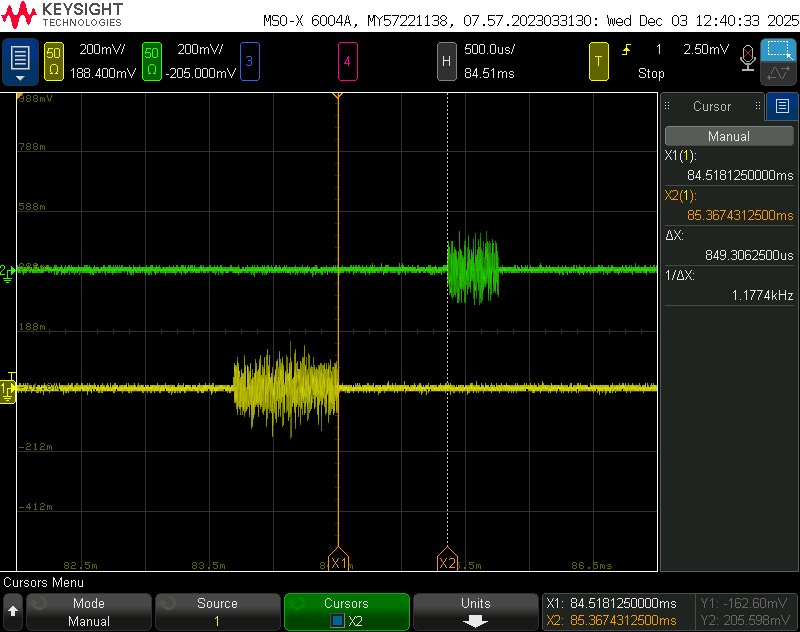
\includegraphics[width=0.8\linewidth]{osceliscope.jpg}
\caption{RX--TX turnaround behavior measured using GPIO timing markers on DSO.}
\end{figure}
\end{frame}

%------------------------------------------------
\begin{frame}{Measured RX--TX Turnaround}
\begin{itemize}
    \item RX--TX turnaround was measured using GPIO markers and DSO.
    \item The measured turnaround delay was approximately:
\end{itemize}

\begin{equation}
T_{\mathrm{turnaround}} \approx 850~\mu s
\end{equation}

\begin{itemize}
    \item This corresponds to nearly two DECT-2020 NR slots.
    \item The delay is dominated by:
    \begin{itemize}
        \item transceiver reconfiguration,
        \item firmware processing,
        \item frame and slot alignment.
    \end{itemize}
\end{itemize}
\end{frame}

%------------------------------------------------
\begin{frame}{Internal Modem Timing Validation}
\begin{itemize}
    \item Internal modem timing was used to cross-check DSO measurements.
    \item One DECT-2020 NR slot corresponds to 28,800 modem ticks.
    \item RX processing takes several hundred microseconds.
    \item TX initiation spans approximately one DECT-2020 NR slot.
    \item These values are consistent with the measured 850 $\mu$s turnaround.
\end{itemize}
\end{frame}

%------------------------------------------------
\section{Discussion}

\begin{frame}{Impact on Industrial Control}
\begin{itemize}
    \item Sensor data and actuator commands are tightly coupled.
    \item Frequent UL/DL alternation increases control-loop latency.
    \item For short-packet traffic, PHY transmission time is not the dominant factor.
    \item Hardware-induced turnaround delay becomes a major bottleneck.
\end{itemize}
\end{frame}

%------------------------------------------------
\begin{frame}{Single-Transceiver Limitation}
\begin{block}{Observation}
The evaluated nRF9151 platform uses a single RF transceiver chain.
\end{block}

\begin{itemize}
    \item This reduces cost and power consumption.
    \item But it forces sequential RX and TX operation.
    \item The resulting turnaround delay cannot be eliminated by scheduling alone.
\end{itemize}
\end{frame}

%------------------------------------------------
\begin{frame}{Design Implications}
\begin{itemize}
    \item Future DECT-2020 NR systems should consider turnaround-aware design.
    \item Possible improvements include:
    \begin{itemize}
        \item separate RX and TX chains,
        \item UL/DL resource separation,
        \item turnaround-aware MAC scheduling,
        \item hybrid TDD/resource allocation modes.
    \end{itemize}
\end{itemize}
\end{frame}

%------------------------------------------------
\section{Conclusion}

\begin{frame}{Conclusion}
\begin{itemize}
    \item This work presented a measurement-driven latency analysis of DECT-2020 NR.
    \item RX--TX turnaround was measured at approximately 850 $\mu$s.
    \item The delay corresponds to nearly two DECT-2020 NR slots.
    \item Turnaround delay is a dominant contributor to latency in short-packet traffic.
    \item Scheduling affects how often the delay occurs, but cannot remove it.
    \item Hardware-aware design is necessary for future low-latency systems.
\end{itemize}
\end{frame}

%------------------------------------------------
\begin{frame}{Main Takeaway}
\centering
\Large
Latency in practical DECT-2020 NR systems is not only a scheduling problem.\\[0.5cm]

\textbf{It is strongly constrained by RX--TX turnaround on single-transceiver hardware.}
\end{frame}

%------------------------------------------------
\begin{frame}{Future Work}
\begin{itemize}
    \item Evaluate multi-chain DECT-2020 NR architectures.
    \item Study UL/DL channel separation.
    \item Develop turnaround-aware scheduling algorithms.
    \item Extend measurements to multi-node industrial scenarios.
    \item Analyze latency under realistic traffic loads.
\end{itemize}
\end{frame}

%------------------------------------------------
\begin{frame}
\centering
\Huge Thank You\\[0.5cm]
\Large Questions?
\end{frame}

%------------------------------------------------
\end{document}